\documentclass{rapport}
\usepackage{lipsum}
% \title{Rapport} %Titre du fichier


\usepackage{hyperref}
\usepackage{matlab-prettifier}
\usepackage{geometry}
\usepackage{verbatim}
\usepackage{afterpage}
\usepackage{algorithm}
\usepackage{graphicx}
\usepackage{natbib}
\usepackage[english]{babel}
\usepackage{listings}
\usepackage{amssymb}
\usepackage{amssymb} 
\usepackage[utf8]{inputenc}
\usepackage{siunitx}
\usepackage{wasysym}
\usepackage{xcolor}
\usepackage{minted} 
\usepackage{svg}
\usepackage{url}


\usepackage{algpseudocode}



\usepackage{rotating} %pour pouvoir faire tourner les images






\begin{document}

\logo{images/FPMs.png}
\unif{}
\titre{Transformers for Time Series Forecasting} %Titre du fichier .pdf
\cours{I-ILIA-202 : Advanced Deep Learning} %Nom du cours
\sujet{Project report} %Nom du sujet

\enseignant{Saïd. \textsc{MAHMOUDI}\
} %Nom de l'enseignant
\assistant{O. \textsc{AMEL}\\
A. \textsc{COOLS}}
\eleves{
Cyril \textsc{TAQUET}\\
Thibaut \textsc{WINDAL}\\


}
		 %Nom des élèves

%----------- Initialisation -------------------
        
\fairemarges %Afficher les marges
\fairepagedegarde %Créer la page de garde
\tabledematieres %Créer la table de matières



% \section*{Abstract}
% \addcontentsline{toc}{section}{Abstract}
% In this paper we are going to do time series forecasting applied on energy consumption. We will be using 4 different well known method: ARIMA, Random Forest, LSTM and Transformer. We compare them on 3 differents task 1 datapoint forecasting, one-day forecasting and the all the test set recursive forecasting. We have found that for long term forecasting LSTM was the best suited model that could predict up to 15 days in advance the consumption while retaining good metrics.

\section*{Abstract}
\addcontentsline{toc}{section}{Abstract}

Time series forecasting plays a crucial role in modeling and predicting energy consumption, where accurate forecasts are essential for planning and operational decision-making. In this paper, we study the problem of electrical energy consumption forecasting and compare four widely used approaches: ARIMA, Random Forest regression, Long Short-Term Memory (LSTM) networks, and Transformer-based models.
\par
The models are evaluated on three forecasting tasks of increasing difficulty: one-step-ahead prediction, one-day-ahead forecasting, and long-term recursive forecasting over the entire test set. Performance is assessed using standard error metrics, including MAE, MASE, and SMAPE.
\par
Our results show that Transformer models achieve the best performance for short-term, one-step-ahead forecasting, while ARIMA struggle in multi-step settings. For long-term recursive forecasting, LSTM models demonstrate superior stability and robustness, maintaining acceptable accuracy for prediction horizons of up to 15 days.


% \section*{Introduction}
% \addcontentsline{toc}{section}{Introduction}

% Time series forecasting (or analysis) is the method used to analyse the time series and forecast the futur evolution of this data. Time series is a special type of data that is composed by a list of point that are taken succesively. It is the most often used to see the evolution of a data in the time. Those data can represent whatever it need to be: failure in a system, price of a stock.


% \par
% In our case, we will applying this principes to forecast of energy consumtion.
% In this rapport we will start to by talking about related work already available in the stat of the art. We will then explain our approach of this problem and explain our experimental setup. We will then finish by our result and an conclusion to sum up everything.


\section*{Introduction}
\addcontentsline{toc}{section}{Introduction}

Time series forecasting is the process of analyzing historical observations collected over time in order to model underlying patterns and predict future values. A time series is a specific type of data composed of sequentially ordered observations, typically recorded at regular time intervals. Such data are widely used to study temporal evolution in a broad range of applications, including system monitoring, financial markets, and demand estimation.

\par
In this work, we focus on the problem of forecasting electrical energy consumption. Accurate energy demand forecasting is a critical task for resource planning, load balancing, and operational decision-making. The temporal nature of consumption data, combined with recurring patterns and long-term trends, makes time series modeling particularly well suited for this application.

\par
This report is structured as follows. First, we review related work and existing approaches from the state of the art. We then describe our methodology and experimental setup, including data preprocessing, model selection, and evaluation metrics. Finally, we present and analyze the experimental results before concluding with a summary of the main findings and perspectives for future work.


% TO DO FINIR INTRO QUAND TOUT FAIT SERA PLUS SIMPLE

% JUSTE DOIT DIRE QUE VA UTILISER 2 MODÈLE NORMAL ET 1 DEEP ET 1 TRANSOFRMER





\section{Related work}
% Time series forecasting is a topic that have been around since at least the 80's and is a subject that can be applied in various domain like our energy consumption but also trading, medicines which mean that a lot reasearch has been done. 
% \par
% Since the 80's a lot informatic has change, research over this subject has also evolved with the new technics found in the rest of the AI research fies I.E that it beeggan with signal processing method and the it evolved to more machine learning process. It also seen a lot of evolution in machine learning starting with random forest, then having MLP (multi layer perceptron), CNN (convolutionnal neural network), RNN (recurant neural network) and finaly transformers. So this mean that we have lot of choice in our model selection\cite{De_Gooijer2006-mi, Hahn2023-rc}.
% \par
% Per stated in the introduction we are going to use different class of model. For each model that we will be using we are going to introduce theoricaly the model and what we expect from it.

% \par
% One of the oldest modal than we can find that has been used a lot is ARIMA which stand for \emph{autoregressive integrated moving average}. This method is based on signal processing and try to mitigate 3 principle toegether : 
% \begin{itemize}
%     \item AutoRegressive : the part that will look at past data
%     \item Integrated : differentiate the serie to make the distribution remain stationnary which elimanted seasonal effect.
%     \item Moving Average : extract relationship between data and residual error. Which is usefull to track short-term changes.
% \end{itemize}
% To find all parameter of this method, it is pretty common to use \emph{Box-Jenkis} method\cite{Shumway2017-kk} but other method also exist and nowadays python libraries implement method to find good parameters.
% \par
% ARIMA model is not perfect so there exist a lot variant that comes to correct a problem. By example SARIMA which allow ARIMA model to be used on stationary time series. \cite{Valipour2015-sv} Staionarity is the property of the dataset to have a constant mean, auto-correlation and variance.

Time series forecasting has been an active area of research since at least the 1980s and has found applications in a wide range of domains, including energy consumption, financial markets, and healthcare. Due to its practical importance, the field has attracted substantial research attention over the past decades.

\par
Since the 1980s, major advances in computing power and data availability have significantly influenced the evolution of time series forecasting methods. Early approaches were primarily based on signal processing and statistical modeling techniques. %Over time, these methods have been progressively complemented—and in some cases replaced—by machine learning and, more recently, deep learning approaches. This evolution mirrors broader developments in artificial intelligence research.

\par
Machine learning methods for time series forecasting have evolved from classical algorithms such as random forests to neural network-based models, including multilayer perceptrons (MLP), convolutional neural networks (CNN), recurrent neural networks (RNN), and, more recently, transformer-based architectures. As a result, a wide variety of models are now available, each with distinct assumptions, strengths, and limitations \cite{De_Gooijer2006-mi, Hahn2023-rc}.

% \par
% As stated in the introduction, this work considers several classes of forecasting models. For each model, we provide a theoretical overview and discuss the expected behavior and performance characteristics. %REVENIR

\par
One of the earliest and most widely used statistical models for time series forecasting is the ARIMA model, which stands for \emph{AutoRegressive Integrated Moving Average}. ARIMA models are rooted in classical time series analysis and are designed to capture temporal dependencies through three main components:
\begin{itemize}
    \item Autoregressive (AR): models the dependence between an observation and a number of its past values.
    \item Integrated (I): applies differencing to the time series in order to achieve stationarity.
    \item Moving Average (MA): models the dependence between an observation and past forecast errors, which is particularly useful for capturing short-term fluctuations.
\end{itemize}

\par
The parameters of an ARIMA model are traditionally identified using the Box--Jenkins methodology \cite{Shumway2017-kk}, although alternative approaches exist. Modern statistical software libraries provide automated procedures for parameter selection.

\par
Despite its effectiveness, the ARIMA model has limitations, particularly when dealing with seasonal patterns. Several extensions have been proposed to address these issues, such as the Seasonal ARIMA (SARIMA) model \cite{Valipour2015-sv}, which explicitly incorporates seasonal components.% Stationarity, in this context, refers to the property of a time series whose statistical characteristics—such as mean, variance, and autocorrelation—remain constant over time.




% \par
% In the deep learning model, there is a lot of model that can be used. Some are bette suited to tackel prediction of timeserie like familiy recusive neural network (RNN)  or the transformer model familiy. 
% \par

% The idea behing the family of RNN is a model that for each timestamp will take a value (or vector) as input. With this, it will update his internal vector that represent the memory of the model. With this memory he can output a vector to predict the next element. By this design it could theoricaly handeld infine long sequence which is interessting\cite{Schmidt2019-kw}. The Figure~(\ref{fig:rnnarchitecture}) show the architecture of this model.

% \begin{figure}[H]
% \centering
% 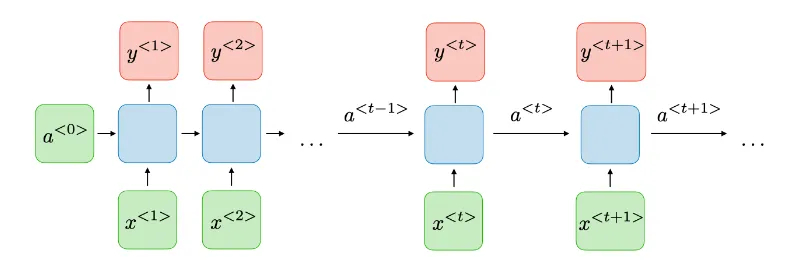
\includegraphics[width=0.80\textwidth]{images/rnn_architecture.jpg}
% \caption{RNN Architecture}
% \label{fig:rnnarchitecture}
% \end{figure}


% In the family of RNN, there is also the model LSTM (Long Short-Term Memory). The there existe different version and the version a bit more advanced is LSTM for long short term memory. This variant arise to counter some limitation of RNN such as vanishing gradient that make it hard to train RNN models on very long series so making hard for to model long term relation ship. Both of this model has still the bottle neck to only have one internal representation. 
% \par


% In the other hand the transformer family that us the concept of attention to avoid unic interal representation that is bottlenecking RNN family. It was at the basis developped for NPL\cite{Vaswani2017-jv}. But a sentence can be represented in a time serie where at each step we have a word. So this principe can easily be reused and has been reused to trackle time series forecasting. 

% \par
% The attention (or self-attention in our case) is a mecanism that is capable of dynamicaly assign importance weight (or attention weight) to different element in the input series. Which completely overcome the bottle neck of having only one representation of memory.
% \par
% By looking at state of the art method used in currently libraries. They claim that it surpass everything that was known\cite{Zerveas2021-ff}. They also talk that those new implementation can be trained with fewer data so we should be able to train the model. 

Among deep learning approaches, several model architectures can be applied to time series forecasting. Some families of models are particularly well suited for sequential data, including recurrent neural networks (RNNs) and transformer-based architectures.

\par
The core idea behind the RNN family is to process sequential data by iteratively updating an internal hidden state. At each time step, the model receives an input value (or vector), which is used together with the previous hidden state to update the internal representation of the sequence. This hidden state serves as a form of memory and can be used to generate an output, such as a prediction of the next time step. Due to this recursive structure, RNNs are, in theory, capable of handling sequences of arbitrary length \cite{Schmidt2019-kw}. Figure~\ref{fig:rnnarchitecture} illustrates the general concept of an RNN.

\begin{figure}[H]
\centering
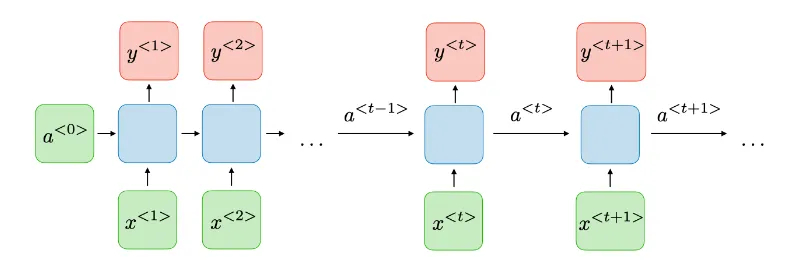
\includegraphics[width=0.80\textwidth]{images/rnn_architecture.jpg}
\caption{Recurrent Neural Network (RNN) concept where $x$ represent the input, $a$ the hidden state and $y$ the output value}
\label{fig:rnnarchitecture}
\end{figure}

\par
Within the RNN family, Long Short-Term Memory (LSTM) networks represent an important extension. Several variants of LSTM architectures exist, all designed to address key limitations of standard RNNs. In particular, LSTMs mitigate the vanishing gradient problem, which makes it difficult for vanilla RNNs to learn long-term dependencies in long sequences. By introducing gating mechanisms, LSTMs are better suited to modeling long-range temporal relationships. However, both RNNs and LSTMs remain constrained by the use of a single hidden-state representation, which can act as a bottleneck when modeling complex dependencies.\cite{Waqas2024-xj}

\par
In contrast, transformer-based models rely on the attention mechanism to overcome this limitation. Originally developed for natural language processing tasks \cite{Vaswani2017-jv}, transformers do not rely on recurrent computations. Instead, they process sequences by allowing each element to directly attend to all other elements in the sequence. Since a sentence can be viewed as a time-ordered sequence of tokens, this framework naturally extends to time series forecasting and has been widely adopted in this context.

\par
The attention mechanism, and more specifically self-attention, dynamically assigns importance weights to different elements of the input sequence. This enables the model to capture both short-term and long-term dependencies without relying on a single compressed memory representation, thereby alleviating the bottleneck inherent in RNN-based models.

\par
Recent state-of-the-art transformer-based models for time series forecasting have demonstrated strong empirical performance and outperform traditional statistical and recurrent neural network approaches \cite{Zerveas2021-ff}. Additionally, they report improved data efficiency compared to earlier deep learning models, making these architectures particularly attractive in practical forecasting settings.
% \section{Proposed approach}
% Beofre looking at any model we have started to look first at the dataset to see the form of data and them look at model that would be best-suited for our model.

% \par
% Our dataset is the \textit{Electricity Diagrams}\cite{electricityloaddiagrams20112014_321} which represent the electric consumption from 370 clients. For each client we have data from begining of 2011 to the end of 2014 and we have a data point every 15 minutes. Which represent over 140 256 data points.
% \par
% The author of this dataset also stated that some of this 370 client were aquired only later than 2011 so there data before the aquiring date is juste defaulted to 0.
% \par
% We were tasked to create a model that is capable of forecasting for only one client. Without any constraint on a specific client we have looked at all client and took a client that was already there since the begining in 2011 to have the maximum data possible. It might be too much data but at least we can reduce it afterwards and don't need to change client for a specific model because we would lack of data.
% \par
% Also the dataset state that there is no missing data but while we were looking at the data we have seen client that were consuming electricity and then no consumption. We also avoid those client due to harsh cut in consumption which ressemble most to a technical difficulty that realy good data.
% \par
% With that in mind we look at every client which minimum consumption is greate than 0. With that we still have a lot of choice of 90 clients and we arbirtraly took the client \textbf{MT\_292}. Figure~(\ref{fig:dataset}) represent it consumption.

% \begin{figure}[H]
% \centering
% 
\includegraphics[width=1\textwidth]{images/dataset.png}
% \caption{Consumption of client 'MT\_292' from 2011 to 2014}
% \label{fig:dataset}
% \end{figure}

% This show that we only have one feature to look: the consumtion. We don't need to look at other factor that could be linked like number of employe or other. We could extract other feature based on the date. We wont try here to extract feature like day of week, or other things in the dataset.

\section{Proposed approach}

Before considering specific forecasting models, an initial analysis of the dataset was conducted in order to understand its structure and determine which modeling approaches would be most appropriate.

\par
The dataset used in this study is the \textit{Electricity Load Diagrams} dataset \cite{electricityloaddiagrams20112014_321}, which contains electricity consumption data for 370 clients. For each client, measurements are recorded at 15-minute intervals from the beginning of 2011 to the end of 2014, resulting in up to 140{,}256 observations per client.

\par
The dataset documentation indicates that some of the 370 clients were added after 2011, and that their consumption values prior to the acquisition date are set to zero. These artificially introduced zero values do not correspond to actual consumption and therefore need to be handled carefully during model selection.

\par
The objective of this work is to construct a forecasting model for a single client. In order to maximize the amount of available training data and ensure consistency across experiments, we considered only clients whose data spans the entire observation period starting in 2011. This choice allows us to later reduce the training horizon if necessary, without having to change the selected client due to data scarcity.

\par
Although the dataset is reported to contain no missing values, exploratory data analysis revealed that some clients exhibit extended periods of zero consumption following non-zero activity. Such abrupt and persistent drops in consumption are likely to reflect data collection issues or atypical behavior rather than realistic usage patterns. Consequently, these clients were excluded from further analysis.

\par
Based on these criteria, we selected clients whose minimum recorded consumption is strictly greater than zero. This filtering step resulted in a subset of 90 clients. From this subset, the client \textbf{MT\_292} was selected for further experimentation. Figure~\ref{fig:dataset} illustrates the electricity consumption of this client over the full observation period.

\begin{figure}[H]
\centering

\includegraphics[width=1\textwidth]{images/dataset.png}
\caption{Electricity consumption of client \textbf{MT\_292} from 2011 to 2014}
\label{fig:dataset}
\end{figure}

\par
For the selected client, the dataset contains a single primary feature: electricity consumption. In this study, we focus exclusively on this univariate time series. While additional features could be derived from the timestamp (e.g., day of the week or time of day), no explicit feature engineering based on calendar information is performed.

\par

% We are going to create model that are capable to forecast one full day which mean 96 new points while looking at some data in the past.
% \par
% We are going to use 4 differents models. The 2 that are the most obvious are LSTM and transformer because they best suited for this kind of problem and have been used in the past for this. 
% \par
% We are considering both because we should have enough data to train transformer but transformer is realy only usefull to capture realy complicated and long relation ship. It might not be required and LSTM model would get nearly as good result while being lighter and requiring less expensive hardware to deploy afterwards.

% \par
% We also want to compare it to simplier machine learning method like ARIMA. Our data is seasonal so SARIMA should be interessint to try. We were not able to train this model due to its complexity being why greater than ARIMA so we had to use ARIMA. We have tried giving only less informations and find that it was trainable with only 1 or 2 week of data which is way less than years. Also a problem of those model is that they are made to predict the next point and will required to use this point to forecast a second point. If the model is not capable of good forecasting we will have that error will accumulate fast.

% \par
% To finish, we also are going to use a Random Forest Regressor. This model is not made at the basis to do timeserie forecasting but we can manipulate while giving a windows as input and output to adapt this model. The idea behind is to see how well we can use a model that is not meant for this task and get good result.

% \par
% Somes metrics are required to be able to compare correctly the model between them. For that we have used :
% \begin{itemize}
%     \item Mean Average Aboslute Error: MAE = $\frac{1}{n}\sum^{n}_{i=1}|y_i-\hat{y}_i|$. It measures directly by how much the forecasting is wrong so it means that is dependant on the size of the data. This metric would not be suited to compare between different clients.
%     \item Mean Average Scalled Absolute Error: MASE = $\frac{\text{MAE}}{\text{MAE}_{\text{naive train}}}$. This metrice normalise MAE by dividing it by the MAE of a naive model (model that just say the last value seen) on the train. If value is better than 1, it mean that we are making a better job than a naive model. 
%     \item Symetric Mean Absolue Error: SMAPE = $\frac{2}{n} \sum_{t=1}^n \frac{\left|y_t-\hat{y}_t\right|}{|y_t|+|\hat{y}_t|}$. Reprensent the percentage of how much any forecast is off.
% \end{itemize}
% In each case, $y$ represent the target value and $\hat{y}$ the predicted value and $n$ is the number of point used to compute the metric. For each metric, the tinier they are the better the model is. 


% \par
% Each model will be evaluated on 3 task: forecasting the next point, forecasting the next day and forecasting the trait in set. The first 2 task is to try the short terme forecasting abilities of our model and the last one is to try the long term forecasting.

% \par
% In advance, we assume that long term forecastin will yield to poor metrics due to error accumulation on long period of time and so for this long term we will also take forecasting at 1 day, 1 week, 1 month and all the dataset to see at which point the error accumulation is too much to be used.


The objective of the proposed models is to forecast electricity consumption over a full day, corresponding to 96 consecutive time steps, using historical observations as input.

\par
Four different forecasting approaches are considered. Among them, Long Short-Term Memory (LSTM) networks and transformer-based models are natural candidates, as they are well suited for sequential prediction tasks and have been successfully applied to time series forecasting in prior work.

\par
Both architectures are evaluated in order to assess the trade-off between model complexity and predictive performance. While transformer models are particularly effective at capturing complex and long-range dependencies, such capabilities may not be strictly necessary for this task. Given the structure of the data, an LSTM model may achieve comparable performance while being computationally lighter and easier to use in practice.

\par
In addition to deep learning approaches, we include classical statistical models as baselines. Since the data exhibits clear seasonal patterns, a Seasonal ARIMA (SARIMA) model would be a natural choice. However, due to the high computational cost and parameter complexity of SARIMA for long time series, we instead employ a standard ARIMA model. Preliminary experiments showed that SARIMA models can be trained using relatively short historical windows (e.g., one to two weeks of data), which is significantly smaller than the full dataset. A known limitation of ARIMA-based approaches is that they are designed for one-step-ahead forecasting; multi-step forecasts therefore require recursive predictions, which can lead to rapid error accumulation.

\par
Finally, a Random Forest Regressor is considered. Although this model is not inherently designed for time series forecasting, it can be adapted to the task by using sliding windows of past observations as input features. This approach allows us to evaluate how well a non-sequential machine learning model performs when repurposed for forecasting tasks.

\par
To enable a fair comparison between models, several evaluation metrics are used:
\begin{itemize}
    \item \textbf{Mean Absolute Error (MAE)}:
    \[
    \text{MAE} = \frac{1}{n}\sum_{i=1}^{n} |y_i - \hat{y}_i|,
    \]
    which directly measures the average magnitude of forecasting errors. Since MAE depends on the scale of the data, it is not suitable for comparing results across different clients.
    
    \item \textbf{Mean Absolute Scaled Error (MASE)}:
    \[
    \text{MASE} = \frac{\text{MAE}}{\text{MAE}_{\text{naive}}},
    \]
    where $\text{MAE}_{\text{naive}}$ corresponds to the MAE of a naive forecasting model that predicts the last observed value used on the train set. Values below 1 indicate an improvement over the naive baseline.
    
    \item \textbf{Symmetric Mean Absolute Percentage Error (SMAPE)}:
    \[
    \text{SMAPE} = \frac{2}{n} \sum_{i=1}^{n} \frac{|y_i - \hat{y}_i|}{|y_i| + |\hat{y}_i|},
    \]
    which expresses forecasting error as a relative percentage.
\end{itemize}

\par
In all cases, $y$ denotes the true target value, $\hat{y}$ the predicted value, and $n$ the number of observations used to compute the metric. Lower values indicate better predictive performance.

\par
Each model is evaluated on three forecasting tasks: one-step-ahead prediction, one-day-ahead forecasting, and long-horizon forecasting over the entire test set. The first two tasks assess short-term predictive performance, while the final task evaluates the models' ability to maintain accuracy over extended horizons.

\par
We anticipate that long-term forecasts will exhibit degraded performance due to the accumulation of prediction errors over time. To further analyze this effect, additional evaluations are conducted at intermediate horizons (one day, one week, one month, and the full test period) in order to identify the point at which error accumulation renders forecasts unreliable.




% \section{Experimental setup}
% One of the key parameter of the work is how we have used the dataset to create our train data to be able to correctly train our model.
% \par
% With LSTM and transformer model we could use the whole serie at one but it would not be very effective. For that, we have decided to use multiple sliding windows to create a dataset. The idea is to have an input window and a forecast window. There name are straigth forward everything in the input window is the input of the model and need to predict the forecast window. Figure~(\ref{fig:dataset_pretraitement}) represent this porcessus.

% \begin{figure}[H]
% \centering
% 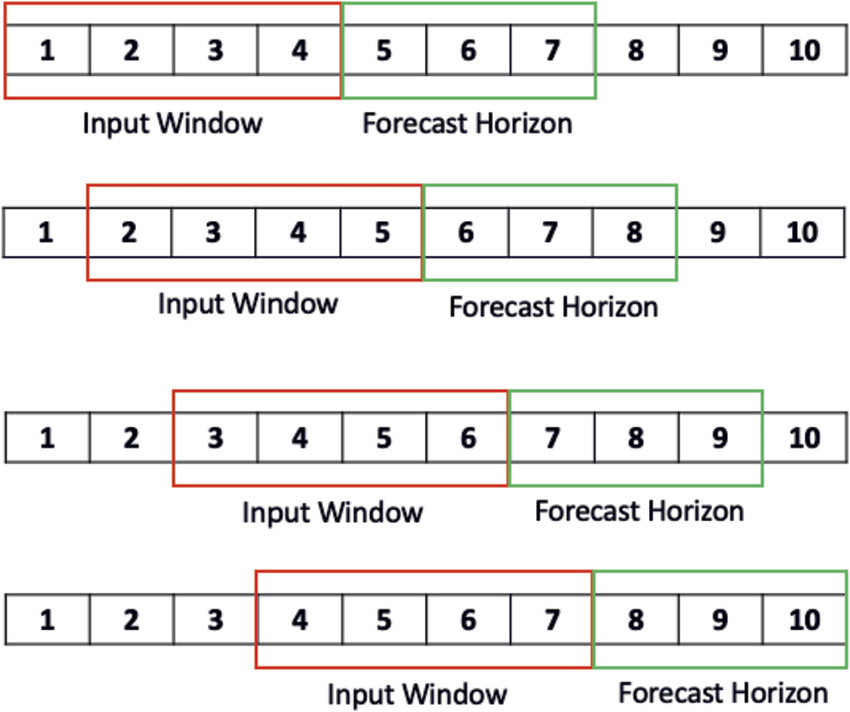
\includegraphics[width=0.6\textwidth]{images/dataset_pretraitement.jpg}
% \caption{Pretraitement of dataset to be used by our model}
% \label{fig:dataset_pretraitement}
% \end{figure}

% We made the input window of size 672 which represent a week of data and forecast for a period of 1 day which is 96 points. 
% \par
% This allow to train of shorter data more variate data at the expense that it impossible to learn relation in the data that is bigger than one week. We found this is okay because the data only evole on long period of time like a year and is most likely linked to something external on the client. There day to day consumption is pretty much similar every day and wanting to forecast those change on long term seams a bit surrealistic.
% \par
% This dataset also allow us to train the random forest regressor that will use this a vector of input and will create a vector of output. Without this, it would impossible to even forecast the anything.



% \par
% We apply this principe on the time series and them we split everything in 3 time series. The first one is used to train the model and take 80\% of the lenght. Then we have 10\% of validation followed by the last 10\% of for test. We have taken the data in the original serie in order above. It does not use random and so is always replicable.
% \par
% The idea is to get data to train model but for that we need verify our parameter with the dataset validation and after all we measure the performance with the test dataset.
% \par

% \par
% This seperation is not applyable on the ARIMA model. It want as input the whole time series. But we still perfomed the train, validation and test split.

% \par
% For the ARIMA model we used library \textit{pmdarima} which proposed a state of the art selection of the best parameter. For the Random Forest Regressor we used \textit{scikit-learn} which is also a state of the art implementation of this method. Those are pretty straitgh forward because they don't have a lot of parameter and trainer is already predone.

% \par
% For the RNN and transformer model, we have use \textit{TSAI} witch is a library that wrap above \textit{pytorch}. We have use the optimizer ADAM to optimize parameter and batch size to load multiple training element at once. 

% \par
% When we could decide the loss function we have used L1 loss function because it is more reliable when we have outlier and as seen in Figure~(\ref{fig:dataset}) we have some. 

% \par
% All our code is avaiable on our github \url{https://github.com/orbitalgamer/Advanced-Deep-Learning}.

\section{Experimental setup}

A key component of this work concerns how the dataset is structured and partitioned in order to train and evaluate the forecasting models in a consistent and reproducible manner.

\par
Although recurrent and transformer-based models are capable of processing long sequences, using the full time series as a single training example is neither efficient nor effective. Instead, we adopt a sliding-window approach to construct the training dataset. Each sample consists of an input window and a corresponding forecasting window. The input window is provided to the model, which is tasked with predicting the values in the forecast window. Figure~\ref{fig:dataset_pretraitement} illustrates this preprocessing procedure.

\begin{figure}[H]
\centering
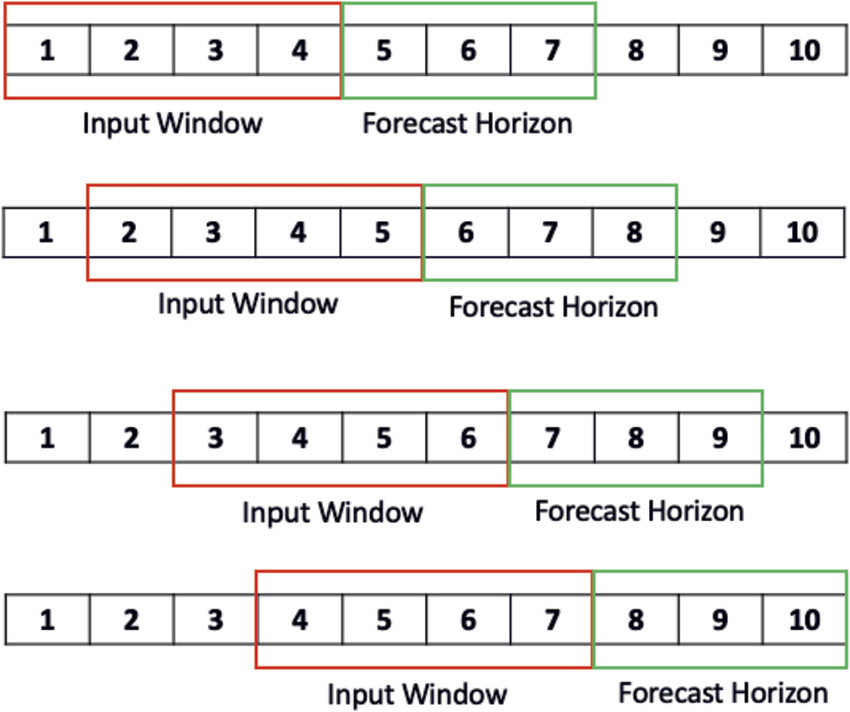
\includegraphics[width=0.6\textwidth]{images/dataset_pretraitement.jpg}
\caption{Sliding-window preprocessing applied to the time series}
\label{fig:dataset_pretraitement}
\end{figure}

\par
The input window length is set to 672 time steps, corresponding to one week of data, while the forecasting horizon is fixed to one day, i.e., 96 time steps. This configuration enables the generation of a large number of training samples from a single time series, thereby increasing data variability during training.

\par
This design choice limits the model’s ability to explicitly capture dependencies spanning more than one week. However, this constraint is considered acceptable in the present context, as long-term consumption trends (e.g., yearly variations) are likely driven by external factors specific to the client. In contrast, daily and weekly consumption patterns are relatively stable and therefore more amenable to short- and medium-term forecasting.

\par
The same sliding-window representation is also used to train the Random Forest Regressor, which requires fixed-size input and output vectors. Without this transformation, applying such a model to time series forecasting would not be feasible.

\par
After window generation, the data is split chronologically into three subsets: 80\% for training, 10\% for validation, and 10\% for testing. The split is performed in temporal order without random shuffling, ensuring that no future information is leaked into the training process and that all experiments are fully reproducible.

\par
The training set is used to fit model parameters, the validation set to tune hyperparameters, and the test set to evaluate final performance.

\par
This data partitioning strategy is not directly applicable to ARIMA-based models, which require a contiguous time series as input. Nevertheless, we retain the same temporal split and evaluate ARIMA forecasts on the validation and test segments in a consistent manner.

\par
For ARIMA modeling, we use the \textit{pmdarima} library, which provides automated and widely used procedures for selecting optimal model parameters. The Random Forest Regressor is implemented using \textit{scikit-learn}, which offers a well-established and efficient implementation with a limited number of tunable hyperparameters.

\par
Recurrent neural networks and transformer-based models are implemented using the \textit{tsai} library, which is built on top of \textit{PyTorch}. WE use \textit{TSTplus} model from \textit{tsai}. Model parameters are optimized using the Adam optimizer, and training is performed using mini-batches to improve computational efficiency.

\par
The L1 loss function is used for training neural network models, as it is more robust to outliers than the L2 loss. This choice is motivated by the presence of occasional high/low-consumption peaks in the dataset, as illustrated in Figure~\ref{fig:dataset}.

\par
All code and experimental configurations are publicly available at \url{https://github.com/orbitalgamer/Advanced-Deep-Learning}.


% \section{Experimental results}

% The first test we made was on forecasting only the next point. To avoidn recreating all model we forecast for the next 96 point and only take the first element. Which lead to the restult in Table~\ref{tab:1stepforecasting}


% \begin{table}[H]
%     \centering
%     \caption{Result of 1 step forecasting}
%     \label{tab:1stepforecasting}
    
    
%     \setlength{\tabcolsep}{6pt}
%     \renewcommand{\arraystretch}{1.1}
    
%     \begin{tabular}{l|c|c|c}
    
%     \hline
%     Method & MAE & MASE & SMAPE \\
%     \hline
%     ARIMA & 18,18     &1,04      &0,078        \\
%     \hline
%     Random Forest & 19,41     & 1,11      & 0,087        \\
%     \hline
%     LSTM & 16,53     & 0,95      &0,072        \\
%     \hline
%     Transformer & 14,55     & 0,8344      &0,063        \\
   
%     \hline
    
%     \end{tabular}
% \end{table}

% We observe here that ARIMA has result that are pretty good. But when we look at is graph on Figure~\ref{fig:arima_forecast} we observe that ARIMA just forecast the last know data point. Which is normal because with the size of data we were not able to put big parameter so that arima can look a lot of data in the past. Metric also look this good because we have a lot of point so we see that difference between an naive forecast and the actual consumption is small. 

% \begin{figure}[H]
% \centering
% 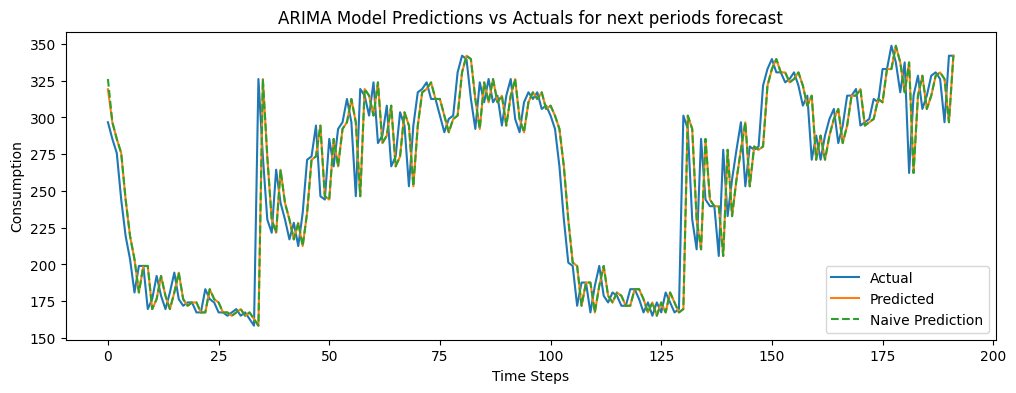
\includegraphics[width=1\textwidth]{images/arima.png}
% \caption{Forecasting of ARIMA method (for the 194 first points)}
% \label{fig:arima_forecast}
% \end{figure}

% For the rest of the result we observe that to forecast the next datapoint, transformer seems to outperform all the others. We also note that only LSTM and Transformer manage to get an MASE score tinir than 1 meaning they are better than just using a naive model which forecast all ways the last known data.

% The second test is on the forecast on a hole day. You can find the restult in the Table~\ref{tab:dayforecasting}.

% \begin{table}[H]
%     \centering
%     \caption{Result of 1 step forecasting}
%     \label{tab:dayforecasting}
    
    
%     \setlength{\tabcolsep}{6pt}
%     \renewcommand{\arraystretch}{1.1}
    
%     \begin{tabular}{l|c|c|c}
    
%     \hline
%     Method & MAE & MASE & SMAPE \\
%     \hline
%     ARIMA & 62,61     & 3,59      & 0,265        \\
%     \hline
%     Random Forest & 22,96     & 1,32      &0,102        \\
%     \hline
%     LSTM & 23,21     &1,33      &0,102        \\
%     \hline
%     Transformer & 23,86     &1,37      &0,107        \\
   
%     \hline
    
%     \end{tabular}
% \end{table}

% With these result we see that model have harder to forecast a day which is not suprising because we need to generate information later in time which could change potentialy a lot. We see that ARIMA is not able to forecast correctly. The few first step is okay and then is just an horizontal line which is realy bad.
% \par
% Now we don't see any paritcular trend if a model is better than another except for arima wich is horrible in comparaison to the 3 other. Random forest was the one that suffered the less from the greater window because it metric did not jump as much as the other models.
% \par
% Remark : MASE metric here I think does not mean anything because we forecast 96 point forward so a naive forecaster won't predict anything but by the definition that is computed on the training set. If we were to compute an MAE naive forecast on the test set we would have score that are close to the MAE value which would lead to have MASE score coser to 0,37 which is significantly better.


\section{Experimental results}

The first experiment evaluates one-step-ahead forecasting performance. In order to avoid retraining separate models, each model is configured to predict the next 96 time steps, and only the first predicted value is retained for evaluation. The resulting performance metrics are reported in Table~\ref{tab:1stepforecasting}.

\begin{table}[H]
    \centering
    \caption{Results of one-step-ahead forecasting}
    \label{tab:1stepforecasting}
    \setlength{\tabcolsep}{6pt}
    \renewcommand{\arraystretch}{1.1}
    \begin{tabular}{l|c|c|c}
    \hline
    Method & MAE & MASE & SMAPE \\
    \hline
    ARIMA & 18.18 & 1.04 & 0.078 \\
    Random Forest & 19.41 & 1.11 & 0.087 \\
    LSTM & 16.53 & 0.95 & 0.072 \\
    Transformer & 14.55 & 0.83 & 0.063 \\
    \hline
    \end{tabular}
\end{table}

\par
ARIMA achieves relatively competitive error metrics in this setting. However, inspection of its forecasts (Figure~\ref{fig:arima_forecast}) reveals that the model  predicts values close to the last observed data point. This behavior is consistent with the limited autoregressive order used, which was constrained by the length of the training window. In addition, the small error magnitude can be partially explained by the high sampling frequency of the data, where consecutive observations tend to be similar, making naive or near-naive forecasts appear effective under one-step evaluation metrics.

\begin{figure}[H]
\centering
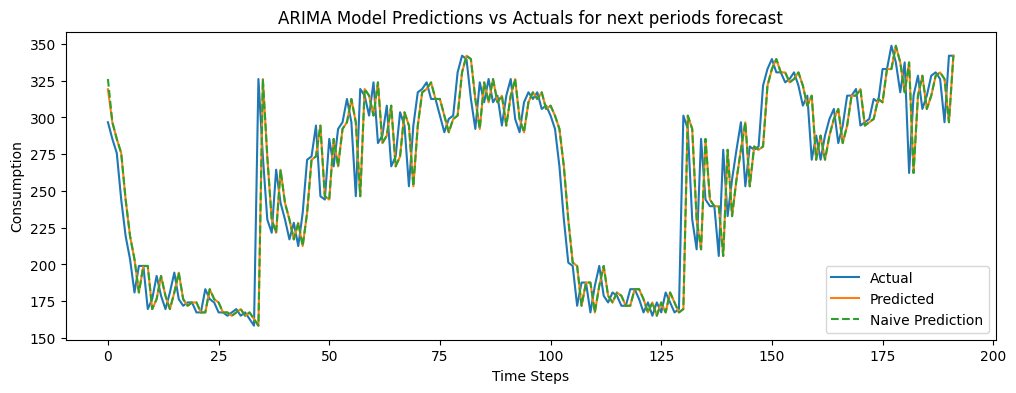
\includegraphics[width=1\textwidth]{images/arima.png}
\caption{One-step-ahead forecasting using the ARIMA model (first 194 points)}
\label{fig:arima_forecast}
\end{figure}

\par
Among the remaining models, the transformer achieves the best overall performance for one-step-ahead forecasting across all metrics. Notably, only the LSTM and transformer models obtain MASE values below 1, indicating performance superior to a naive persistence baseline.

\par
The second experiment evaluates multi-step forecasting over a full day (96 time steps). The corresponding results are presented in Table~\ref{tab:dayforecasting}.

\begin{table}[H]
    \centering
    \caption{Results of one-day-ahead forecasting}
    \label{tab:dayforecasting}
    \setlength{\tabcolsep}{6pt}
    \renewcommand{\arraystretch}{1.1}
    \begin{tabular}{l|c|c|c}
    \hline
    Method & MAE & MASE & SMAPE \\
    \hline
    ARIMA & 62.61 & 3.59 & 0.265 \\
    Random Forest & 22.96 & 1.32 & 0.102 \\
    LSTM & 23.21 & 1.33 & 0.102 \\
    Transformer & 23.86 & 1.37 & 0.107 \\
    \hline
    \end{tabular}
\end{table}

\par
As expected, forecasting performance degrades for all models when predicting a full day ahead, reflecting the increased uncertainty associated with longer forecasting horizons. The ARIMA model performs particularly poorly in this setting, as errors accumulate rapidly during recursive multi-step prediction. While the initial forecasted steps are reasonable, the model quickly converges to constant predictions, resulting in large overall errors.

\par
Among the remaining approaches, no single model clearly dominates across all metrics. However, the Random Forest Regressor exhibits the smallest relative degradation in performance when transitioning from one-step to one-day forecasting, suggesting greater robustness to increasing prediction horizons in this experimental setup.

\par
% It is worth noting that the interpretation of the MASE metric in the multi-step forecasting setting is less straightforward. Since MASE is normalized using the error of a one-step-ahead naive model computed on the training set. The idea behind this metric is to see if the model is better than a naive forecaster. So if we apply a naive forecaster on this test dat while only knowing the first element, it will just predict this element over and over which would yield to an MAE score way higher that would led to MASE way smaller. As shown before, the ARIMA is not realy far from the naive forcast and has an MAE of 62,61. With that in mind we can say that MASE for other model should be around 0,35-0,40 which is considerably better.







% Now for the long term forecasting, you can find all the restult in the Figure~\ref{fig:maelongtermforecast},\ref{fig:maselongtermforecast} and \ref{fig:smapelongtermforecast}. You can see in those graphs that the metric quickly rise up which mean that we have error accumulating. As shown before our model are not perfect to generate the data for a day and now we reuse this data thus making a lot of error accumulation.



% \begin{figure}[H]
% \centering
% 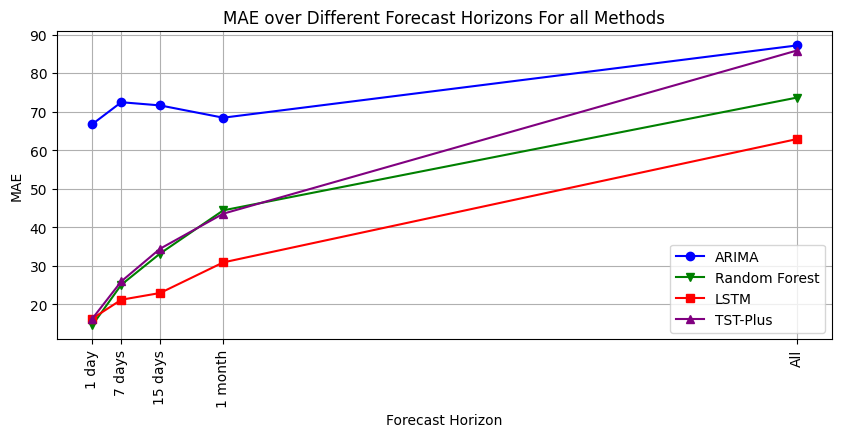
\includegraphics[width=1\textwidth]{images/MAE_longterm_forecasting.png}
% \caption{Evolution of MAE for different forecasating periode for each model}
% \label{fig:maelongtermforecast}
% \end{figure}

% \begin{figure}[H]
% \centering
% 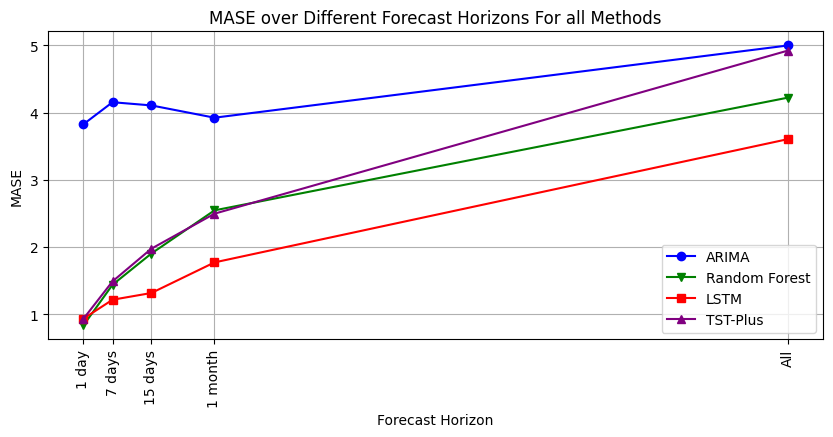
\includegraphics[width=1\textwidth]{images/MASE_longterm_forecasting.png}
% \caption{Evolution of MASE for different forecasating periode for each model}
% \label{fig:maselongtermforecast}
% \end{figure}

% \begin{figure}[H]
% \centering
% 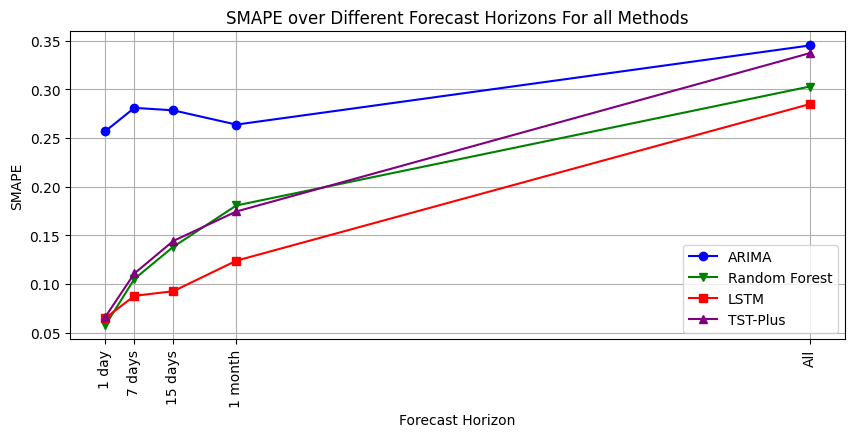
\includegraphics[width=1\textwidth]{images/SMAPE_longterm_forecasting.png}
% \caption{Evolution of SMAPE for different forecasating periode for each model}
% \label{fig:smapelongtermforecast}
% \end{figure}
% \par
% On all this model, LSTM appear to be better than all other model for long term forecasting with this mecanisme of recusrive forecasting. But in aboslute those metrics are okay until days 15 of forecasting. It is said that SMAPE metric under 10\% are considered higly accurate, and up to 20\% is considered somewhat accurate\cite{Makridakis2000-ml}. The Figure~\ref{fig:lstmlongterm} show the forecast for the first 30 day. Eventhough metric says it could be okay ot use up to 30 days we would not forecast for period greater than 15 days.


% \begin{figure}[H]
% \centering
% 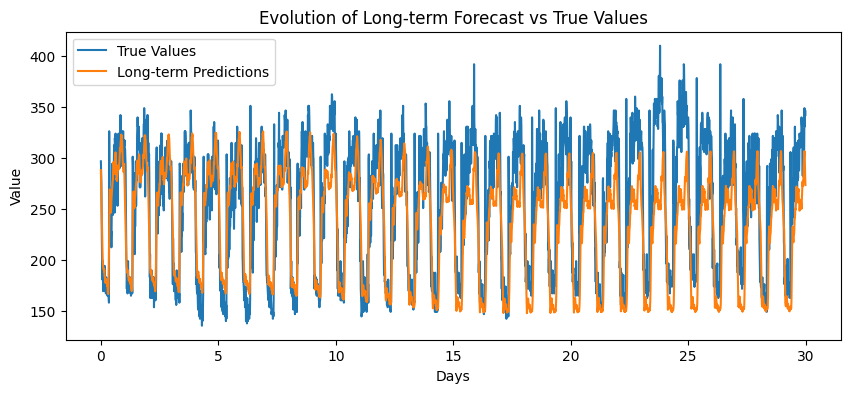
\includegraphics[width=1\textwidth]{images/lstm.png}
% \caption{Evolution of Long-term Forecast in comparaison to true value}
% \label{fig:lstmlongterm}
% \end{figure}

It is important to note that the interpretation of the MASE metric becomes less straightforward in a multi-step forecasting setting. By definition, MASE is normalized using the error of a one-step-ahead naive forecasting model computed on the training set. The primary purpose of this metric is to assess whether a forecasting model outperforms a simple persistence baseline.

\par
In the context of long-horizon forecasting, this normalization can be misleading. If a naive forecaster is applied to the test set while only observing the first value of the forecasting horizon, it will repeatedly predict this value for all subsequent time steps. Such behavior would result in a substantially larger MAE over a 96-step horizon, and consequently yield much smaller MASE values when used as a normalization baseline.

\par
As discussed previously, the ARIMA model produces forecasts that are close to a naive persistence strategy and achieves an MAE of 62.61 for one-day-ahead forecasting. Under this perspective, the effective MASE values for the remaining models would be expected to lie approximately in the range of 0.35 to 0.40, indicating significantly better performance relative to a naive multi-step baseline.

\par
Long-term forecasting performance is illustrated in Figures~\ref{fig:maelongtermforecast}, \ref{fig:maselongtermforecast}, and \ref{fig:smapelongtermforecast}. These figures show a rapid increase in error metrics as the forecasting horizon grows, highlighting the accumulation of prediction errors inherent to recursive forecasting strategies. Since predicted values are reused as inputs for subsequent predictions, even small inaccuracies can compound over time.

\begin{figure}[H]
\centering
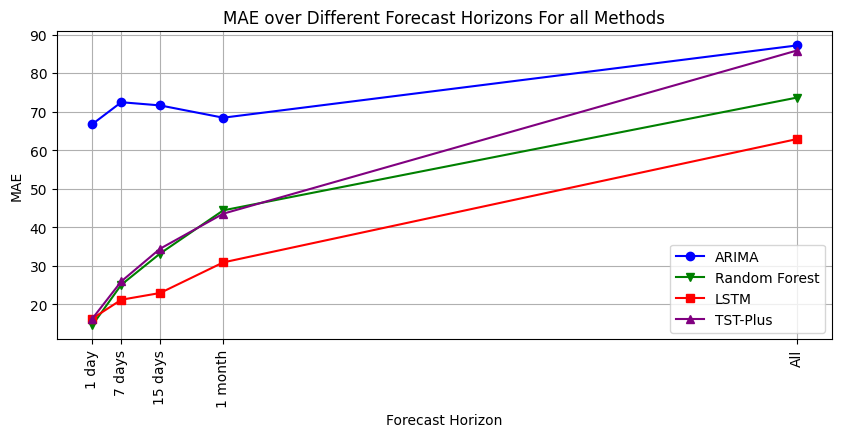
\includegraphics[width=0.85\textwidth]{images/MAE_longterm_forecasting.png}
\caption{Evolution of MAE across different forecasting horizons for each model}
\label{fig:maelongtermforecast}
\end{figure}

\begin{figure}[H]
\centering
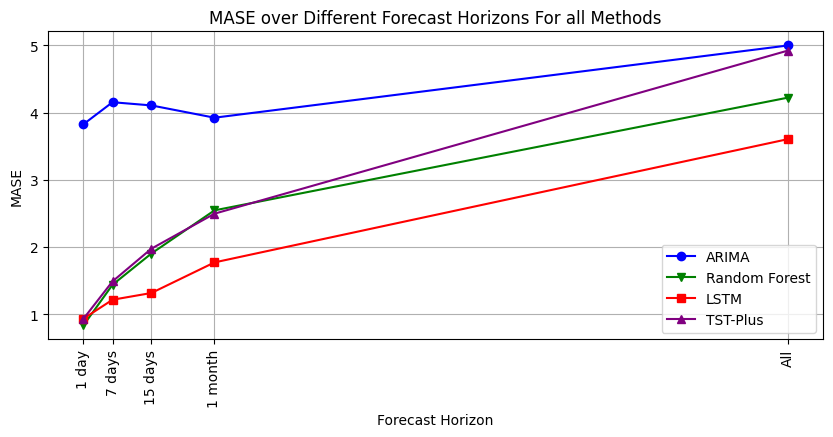
\includegraphics[width=0.85\textwidth]{images/MASE_longterm_forecasting.png}
\caption{Evolution of MASE across different forecasting horizons for each model}
\label{fig:maselongtermforecast}
\end{figure}

\begin{figure}[H]
\centering
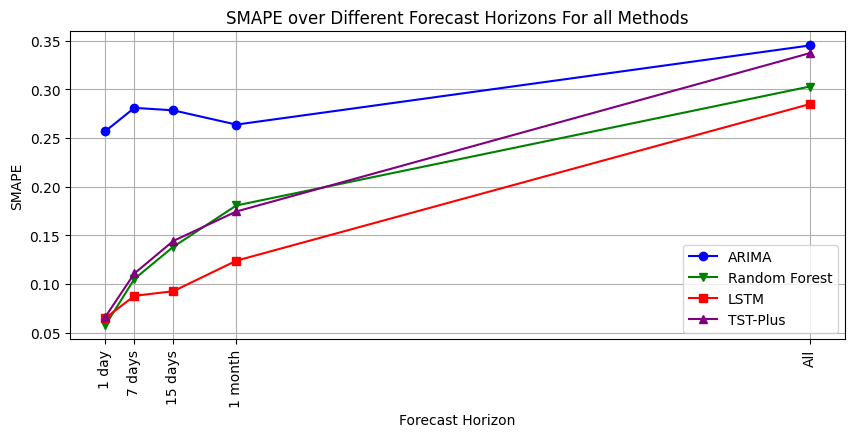
\includegraphics[width=0.85\textwidth]{images/SMAPE_longterm_forecasting.png}
\caption{Evolution of SMAPE across different forecasting horizons for each model}
\label{fig:smapelongtermforecast}
\end{figure}

\par
Among all evaluated models, the LSTM consistently demonstrates superior robustness for long-term forecasting under a recursive prediction scheme. Nevertheless, absolute performance metrics remain within acceptable ranges only up to approximately 30 days ahead. According to commonly used interpretative guidelines, SMAPE values below 10\% are considered highly accurate, while values up to 20\% are regarded as moderately accurate \cite{Makridakis2000-ml}.

\par
Figure~\ref{fig:lstmlongterm} presents the LSTM forecast over the first 30 days. Although the error metrics suggest that predictions may remain usable beyond 15 days, we would conservatively limit the practical forecasting horizon to two weeks, beyond which uncertainty becomes increasingly pronounced.

\begin{figure}[H]
\centering
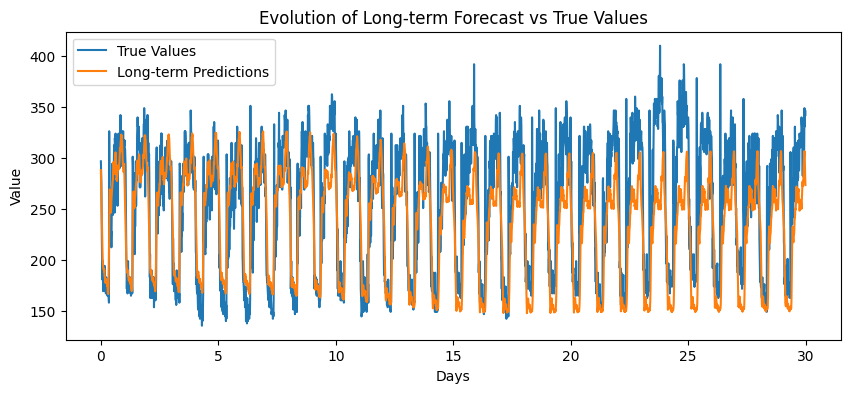
\includegraphics[width=0.9\textwidth]{images/lstm.png}
\caption{Long-term LSTM forecasts compared to ground truth}
\label{fig:lstmlongterm}
\end{figure}



% \section*{Conclusion}
% \addcontentsline{toc}{section}{Conclusion}
% To sum up this arictle. We have tested 4 algorithm in 3 big families: ARIMA and Random forest in classical machine learning alorgithm, LSTM in the recuren model family and a transformer.
% \par
% All this model were trained on the next day forecasting while having as input a full week of data.
% \par
% Theorical studies implied that the best result should have been the transformer. Which we were able to confirm on our task of forecasting the next data point. But transformer rapidly became worse the longer we forecasted. 
% \par
% On our next day forecasting we have that besides ARIMA all models had the same capabilities. But when trying on long term forecasting with recursive usage of the forecasted value, we observed that LSTM was better suited for this task.
% \par
% With our analysis we have seen that LSTM could be use to 30 days of forecasting but we would not recommend to go beyond 15 days.
% \par
% As future perspective for this work. It would be great to try using bigger forecasting windows. We mean by that that our model only predict one full day a the time so it need to reuse this predicted value to get to 15 days. We might get better result with a model that would predict maye 2 or 5 days of data at once.
% \par
% Due to material constraint, we need to reduce the number of parameter and epoch on the transformer model. Maybe with better training you could get better result.
\newpage
\section*{Conclusion}
\addcontentsline{toc}{section}{Conclusion}

This work presented a comparative study of four forecasting approaches drawn from three major model families: classical statistical and machine learning models (ARIMA and Random Forest), recurrent neural networks (LSTM), and transformer-based architectures.

\par
All models were trained to perform one-day-ahead forecasting (96 time steps) using a one-week historical input window. Their performance was evaluated across multiple forecasting horizons, including one-step-ahead, one-day-ahead, and long-term recursive forecasting.

\par
From a theoretical perspective, transformer-based models are expected to deliver superior performance due to their ability to capture complex temporal dependencies. This expectation was confirmed for the one-step-ahead forecasting task, where the transformer achieved the lowest error across all evaluated metrics. However, performance degraded more rapidly for longer forecasting horizons.

\par
For one-day-ahead forecasting, all models except ARIMA exhibited comparable performance, suggesting that short-term daily consumption patterns can be effectively captured by a variety of modeling approaches. In contrast, long-term recursive forecasting revealed clearer differences between models, with the LSTM consistently demonstrating greater robustness to error accumulation.

\par
Although quantitative metrics indicate that LSTM-based forecasts may remain usable for horizons of up to 30 days, a conservative operational limit of approximately 15 days is recommended, beyond which uncertainty and accumulated error become substantial.

% \par
% Several avenues for future work emerge from this study. One promising direction is the use of longer forecasting windows, where models predict multiple consecutive days simultaneously rather than relying on recursive one-day-ahead predictions. Such an approach could reduce error propagation and improve long-horizon forecasting performance.
% Secondly, feature engineering might also be good to explore to give multiple source of information at the model.

% \par
% Finally, due to computational constraints, the transformer model was trained with a reduced number of parameters and training epochs. Future experiments with increased model capacity and extended training may further improve transformer performance and provide a more comprehensive comparison between architectures.


\par
Several avenues for future work emerge from this study. One promising direction is the use of longer forecasting windows, where models predict multiple consecutive days simultaneously rather than relying on recursive one-day-ahead forecasting. Such an approach could reduce error propagation and potentially improve long-horizon forecasting performance.

\par
Another important direction concerns feature engineering. Incorporating additional explanatory variables, such as calendar-based features (e.g., day of the week or seasonality indicators), could provide the models with richer contextual information and lead to more accurate forecasts.

\par
Finally, due to computational constraints, the Transformer model was trained with a limited number of parameters and training epochs. Future experiments using larger model capacities and longer training schedules may further improve Transformer performance and allow for a more comprehensive comparison between deep learning architectures.


\newpage
\section*{Bibliographie}
\addcontentsline{toc}{section}{Bibliographie}
\bibliographystyle{plain}
\bibliography{BB}


% \newpage
\section{Annexes}
\label{Annexes}

\subsection{Illustration Type de Jeux vidéos}



Jeu de course

\begin{figure}[H]
\centering
\includegraphics[width=0.65\textwidth]{images/Super_Mario_Kart_screen_shot.jpg}

\end{figure}

Jeu de Plateau
\begin{figure}[H]
\centering
\includegraphics[width=0.65\textwidth]{images/7952a79aeab9ab44_1200xH.jpg}

\end{figure}
Jeu de stratégie

\begin{figure}[H]
\centering
\includegraphics[width=0.65\textwidth]{images/BOSscreen.png}

\end{figure}

Openworld

\begin{figure}[H]
\centering
\includegraphics[width=0.65\textwidth]{images/008.png}

\end{figure}


\begin{figure}[H]
\centering
\includegraphics[width=0.65\textwidth]{images/images.jpg}

\end{figure}

\subsection{Version antécédentes des maps}
\label{VersionAntMap}
\subsubsection{Infirmerie}
\begin{figure}[H]
\centering
\includegraphics[width=0.65\textwidth]{images/Infirmerie V2.png}
\caption{Première version}
\end{figure}
\subsubsection{marchand}
\begin{figure}[H]
\centering
\includegraphics[width=0.65\textwidth]{images/Marchand V2.png}
\caption{Première version}
\end{figure}
\subsubsection{Donjon}
\begin{figure}[H]
\centering
\includegraphics[width=0.65\textwidth]{images/DonjonV2.png}
\end{figure}


\end{document}

%% report strucutre
% Introduction w/ team
% Architecture
% possible theats  -> vulnerabilities put into place
% vulnerbalities left
% conclusion